% !TeX root = ../Tempel-Daniel.tex

\chapter{Agent Evaluation, Observability and Reliability}

\label{chap:evaluation}

The previous chapters extended the AI Software Engineering Assistant from an LLM into a system that retrieves context, executes tools, maintains task state and operates under production and security constraints. Evaluating only the model is therefore insufficient. A plausible response may accompany an incorrect repository state, missing verification or a policy violation. The relevant unit of evaluation is the complete task execution, including the model, agent harness, retrieval, tools, dependencies and resulting environment state.

A \textbf{task} defines the input, initial environment and success criteria, while one execution is a \textbf{trial}. Each trial produces an \textbf{outcome} and an execution \textbf{trajectory}. Task success may depend on both: the required outcome must be achieved and mandatory execution constraints must be satisfied. \textbf{Observability} records what occurred during the trial, while \textbf{reliability} measures whether successful behaviour is reproduced across comparable trials.

\section{Evaluating complete agent tasks}

For \emph{Fix GitHub issue \#42 and verify the solution}, an evaluation can start from a specified repository revision, issue description, assistant configuration and isolated environment. The assistant operates through the same retrieval and tool interfaces used normally, so the evaluation covers the model and agent harness as a combined system \parencite{grace2026evals}.

A \textbf{grader} evaluates the final code state and mandatory execution constraints. Outcome criteria may require issue-specific tests, regression tests and a successful build; execution criteria may require final verification or prohibit particular operations. Overall success requires all mandatory checks to pass.

For objective software-engineering tasks, deterministic graders such as tests, builds, static analysis and state comparisons are preferable because they provide reproducible evidence. Model-based or human graders remain useful when requirements cannot be represented reliably in code. SWE-bench follows the same outcome-oriented principle by verifying changes to real repositories through execution rather than judging whether a generated patch appears plausible \parencite{jimenez2024swebench}.

Final grading should apply evaluator-controlled checks to the submitted artefact. Intermediate \texttt{run\_tests} feedback is insufficient: the assistant may modify tests or edit code after verification. Independent grading prevents such changes from silently redefining the acceptance criteria.

As established in Chapters~\ref{chap:tool-use} and~\ref{chap:agents}, a failing assertion is a valid tool observation, whereas an invalid request or execution failure is a different event. Evaluation metrics should retain these categories separately.

Evaluation infrastructure requires a similar distinction. A broken grader can make a trial invalid and should be reported separately. In contrast, failures of dependencies that belong to the evaluated deployment remain part of end-to-end reliability. Attempted, invalid and valid unsuccessful trials should therefore remain distinguishable.

Figure~\ref{fig:assistant-trial-evaluation} separates grading of trial outcomes and trajectories from trace-based operational measurements; telemetry alone does not establish task success.

\begin{center}
\begin{minipage}{\linewidth}
\centering
\captionsetup{hypcap=false}
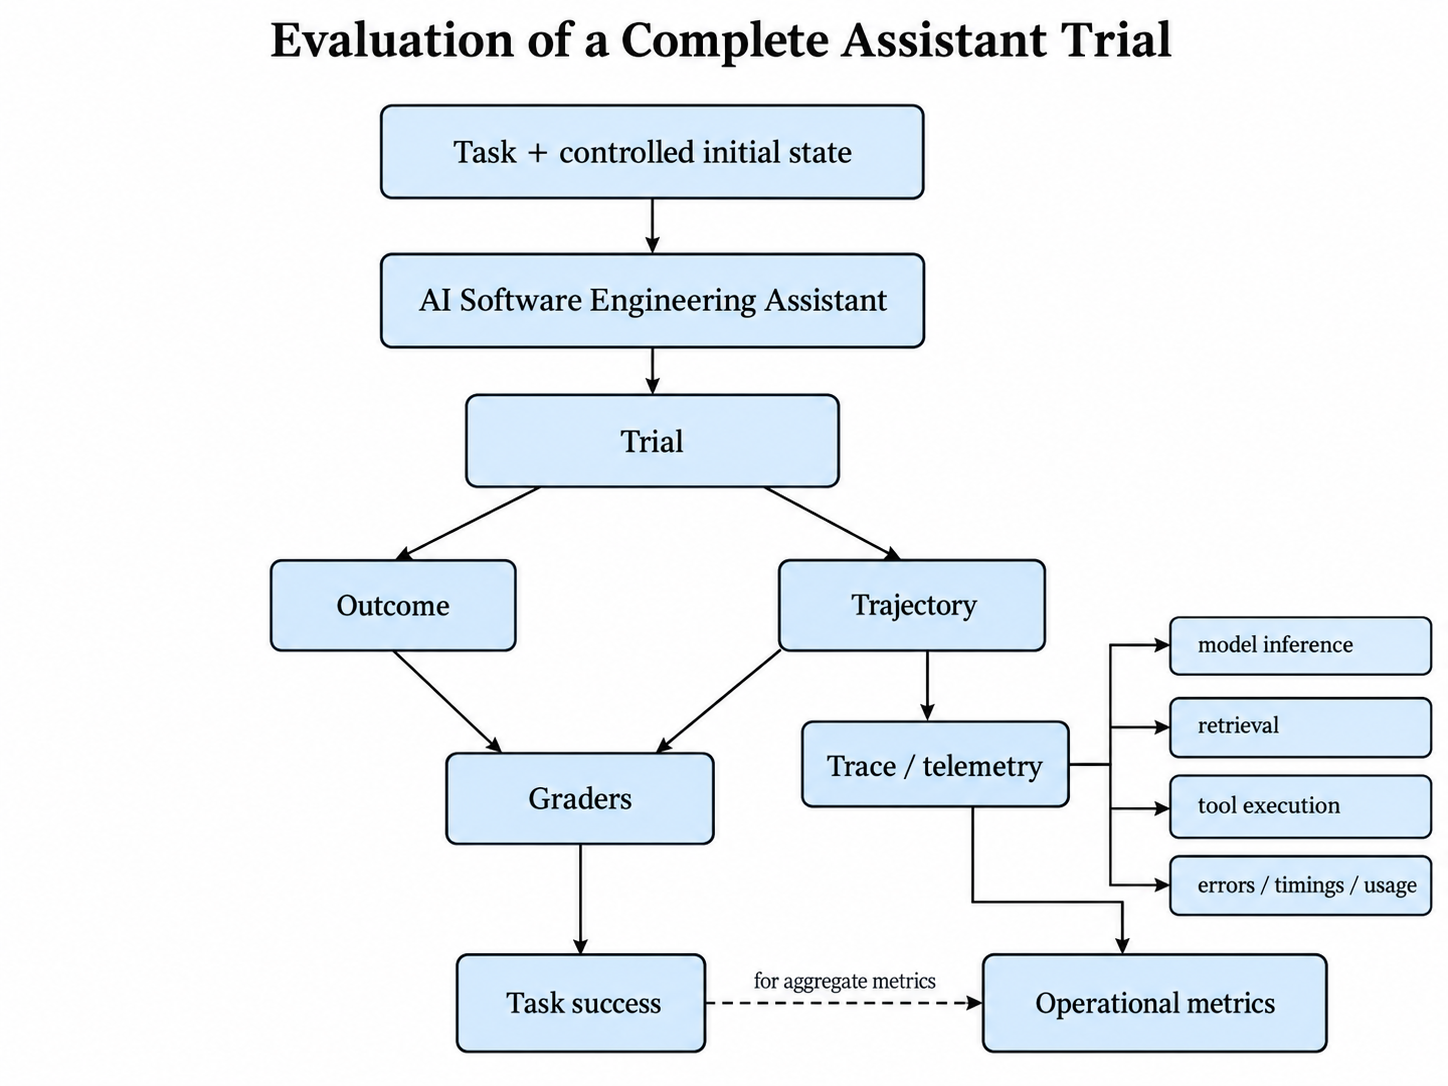
\includegraphics[width=\linewidth]{images/assistant-trial-evaluation.png}
\captionof{figure}{Evaluation and observation of a complete trial of the AI Software Engineering Assistant.}
\label{fig:assistant-trial-evaluation}
\end{minipage}
\end{center}

\section{Trajectories, traces and operational quality}

Task success does not fully describe execution quality. Two trials may produce the same valid patch while requiring very different amounts of inference, tool execution and recovery. The \textbf{trajectory} captures the model decisions, tool requests, observations and state changes that produced the outcome.

Trajectory constraints are useful when the execution path affects correctness or policy compliance, for example when final verification is mandatory or a destructive operation is prohibited. Exact trajectory matching is usually too restrictive because several valid action sequences may produce the same correct outcome. Grading should therefore constrain task-relevant behaviour rather than prescribe an arbitrary sequence of tool calls \parencite{grace2026evals}.

A \textbf{trace} makes the trajectory observable through related spans for retrieval, model inference and application-controlled tool execution. For issue \#42, these may include retrieval, \texttt{read\_file}, \texttt{apply\_patch}, test execution, a corrective model call and final verification. Spans can record duration, status, errors, token usage and operation-specific metadata. OpenTelemetry's GenAI Semantic Conventions provide an emerging vocabulary for such telemetry, although the relevant agent conventions remain under Development in 2026 \parencite{otel-agent-spans}.

Trace analysis can attribute unsuccessful trials to retrieval, model decisions, tool execution, infrastructure or premature termination. These categories support diagnosis and comparison beyond an aggregate task-success rate.

Operational measurements should use the task as their boundary. \textbf{End-to-end task latency} captures the complete execution rather than one model call. Its measurement should define whether queueing, retries, approval waits and final verification are included, and comparisons should use the same definition. Tail metrics such as p95 should also state which trials are included so that excluding timeouts does not make latency appear better while reliability worsens.

Cost requires the same consistency. A trial may consume several model calls, retrieval operations, external services and infrastructure resources. For local inference, compute consumption can replace API charges, but the accounting rule should remain consistent. A useful metric is \textbf{cost per successful task}:

\[
C_{\text{success}} =
\frac{\text{total cost of evaluated trials}}
{\text{number of successful trials}}
\]

It includes resources consumed by unsuccessful trials and should only be compared across equivalent task sets and accounting rules. Together with task success, useful measurements include end-to-end latency, token usage, model and tool invocation counts, infrastructure failures and task-level cost.

A trace supports diagnosis but does not by itself reproduce a failure. Reproduction may also require the repository revision, assistant configuration, retrieval state and relevant external-service state. Distributed or resumed trials may span multiple traces, so telemetry should be correlated with a stable trial identifier. Trace collection must also respect the access-control and secret-handling principles established in the previous chapter.

\section{Reliability and regression evaluation}

A successful trial shows that the assistant solved a task once, not that it will do so consistently. Model sampling, retrieved context and subsequent tool decisions can produce different trajectories from the same initial task. Reliability evaluation therefore repeats tasks under controlled conditions.

Repeated trials should start from the same defined initial state, use comparable execution budgets and not inherit patches or task memory from earlier trials. Corrections made during one execution remain part of that trial; restoring the initial state begins a new one.

This separates \textbf{capability} from \textbf{reliability}. Capability asks whether the assistant can solve a task, while reliability asks whether it does so consistently. \(\tau\)-bench expresses this distinction through \(\mathrm{pass}@k\) and \(\mathrm{pass}^{k}\) for repeated executions of tool-using agents \parencite{yao2024taubench}:

\[
\mathrm{pass}@k = P(\text{at least one of } k \text{ trials succeeds})
\]

\[
\mathrm{pass}^{k} = P(\text{all } k \text{ trials succeed})
\]

A high \(\mathrm{pass}@k\) shows that a successful execution occurs among several attempts, but not that the deployed system can identify the correct attempt. For workflows expected to succeed without such external selection, repeated-trial consistency is therefore important. Comparisons should use the same number of trials and comparable conditions.

Likewise, if 83 of 100 evaluation tasks succeed, 83\% is an observed result on that sample rather than a guaranteed production probability. Small differences between configurations should not automatically be treated as improvements without sufficient evidence to separate systematic changes from run-to-run variation.

Reliability must also survive system changes. Replacing the model or modifying prompts, retrieval, tools or the agent harness may improve some tasks while breaking previously successful behaviour. \textbf{Capability evaluations} probe what the assistant can currently solve, whereas \textbf{regression evaluations} protect behaviour already expected to remain stable \parencite{grace2026evals}.

A production failure can become a regression case. Its trace supports diagnosis, while reproduction additionally requires relevant inputs, configuration and environment state. If the original conditions cannot be reconstructed exactly, a controlled scenario can preserve the behaviour that needs to be tested. After the system is corrected, the case remains in the regression suite for future versions.

Regression cases should still be complemented by capability or held-out tasks, since repeated optimisation against known cases does not independently demonstrate generalisation.

Figure~\ref{fig:evaluation-regression-loop} connects release evaluation with production feedback: diagnosed failures become reproducible cases that test subsequent assistant versions.

\begin{center}
\begin{minipage}{\linewidth}
\centering
\captionsetup{hypcap=false}
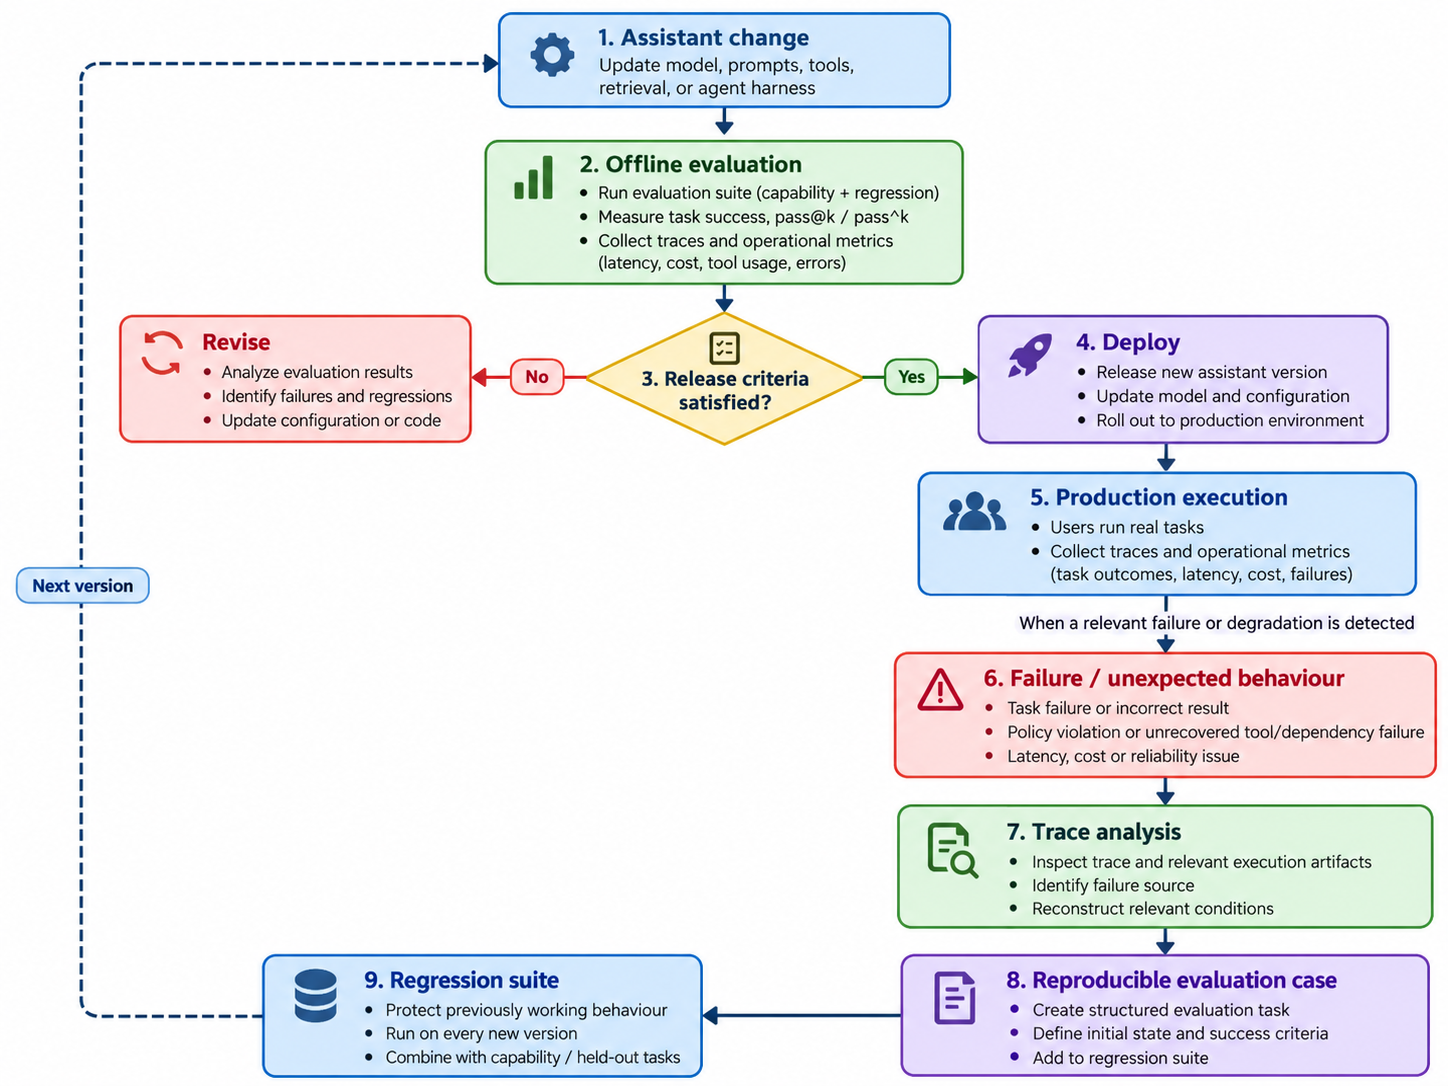
\includegraphics[width=\linewidth]{images/evaluation-regression-loop.png}
\captionof{figure}{Evaluation, release and regression feedback loop.}
\label{fig:evaluation-regression-loop}
\end{minipage}
\end{center}

This creates a closed evaluation loop around the complete assistant. Outcome and mandatory execution checks determine task success; traces expose how the result was produced; task-level latency and cost describe operational performance; repeated trials measure consistency; and regression evaluations protect established behaviour across system changes. Production failures can then become new evaluation cases, allowing the AI Software Engineering Assistant to be assessed as a complete stochastic, tool-using software system rather than only as an LLM.
